\documentclass{jsarticle}

\usepackage{graphicx}
\usepackage{latexsym}
\usepackage{amsmath}
\usepackage{amssymb}
\usepackage{amsthm}
\usepackage{url}
\usepackage{algorithm}
\usepackage{algorithmicx}
\usepackage{algpseudocode}
\newcommand{\argmin}{\operatornamewithlimits{argmin}}
\newcommand{\dd}{\mathrm{d}}
\newcommand{\ee}{\mathrm{e}}

\theoremstyle{definition}
\newtheorem{thm}{定理}
\newtheorem{defi}[thm]{定義}
\newtheorem{prop}[thm]{命題}
\newtheorem{cor}[thm]{系}
\newtheorem{asm}[thm]{仮定}

\renewcommand{\algorithmicrequire}{\textbf{Input:}}
\renewcommand{\algorithmicensure}{\textbf{Output:}}

\title{質問者のプライバシーを保護する特許データベース検索 \\(文献紹介)}
\author{中川研究室 修士2年 胡 瀚林\\指導教員: 中川 裕志 教授}
\date{2016年7月1日}

\begin{document}
\maketitle
\begin{abstract}
企業が特許を取る前に,類似な特許が既に存在するかを確かめるために特許データベースを検索する必要がある.
しかし,検索の質問から企業秘密が漏洩する可能性がある.
また一般的なウェブテキスト検索と違い,特許データベース検索は長い検索質問を用いて検索の精度と再現率を重視している.
紹介文献\cite{pang_embellishing_2010}では直接質問者の質問にデミー単語を混ぜて質問のある種の匿名性を保証し,準同型暗号を用いて真の質問単語だけの関連性スコアを計算できる検索スキームより検索の精度と再現率を維持する.

本発表では\cite{pang_embellishing_2010}を紹介して,LSIを用いる攻撃手法を提案し,特許データベースを用いて提案手法を評価する.
\end{abstract}

\section{はじめに}
テキスト検索をするとき,検索質問をサーバー側に渡さなければならない.しかし,検索質問からユーザーの情報が漏洩する危険があることがAOL事件\cite{_face_2006}より証明された.特に特許検索の場合は質問が研究開発動向などは企業秘密を含んでいるため,一般的なウェブ検索のユーザーよりテキスト検索のプライバシー問題を重視している.

今テキスト検索エンジンの大半が類似検索である.全ての質問単語を含んでいる文章しか検索できないキーワード検索と違い,類似検索は文章と質問の関連性を計算し文章にランクをつける\cite{zobel_inverted_2006}.毎回全ての文章との関連性を計算しないために検索エンジンが単語と文章の関連値を転置ファイルに保存し,質問の単語と文章の関連値の和を質問とその文章の関連性とする.このような計算が必要であるため,\cite{bethEourt_new_2006},\cite{freedman_keyword_2005},\cite{boneh_public_2004},\cite{song_practical_2000}などキーワード検索だけ対応できる研究は類似検索に応用できない.また質問のある種の匿名性より質問者のプライバシーを保護する手法がある.\cite{murugesan_providing_2009}では事前的に静的な質問セットを作り,真の質問$q$の代わりに真のと一番類似な質問$q'$を含んでいる質問セットをサーバーに送る.$q'$が真の質問の大半な結果を検索できると考えられ,質問セット中の他の質問をダミー質問にする.そのため,このメカニズムは検索の精度と再現率に影響を大きく与える.また,質問の長さの増加と伴って質問の可能な組み合わせが指数的に増加するため,実践的には特許検索など長い質問が多いテキスト検索と質問拡張\cite{qiu_concept_1993,xu_query_1996}に対応できない.

\cite{pang_embellishing_2010}では長い質問と類似検索に対応できるメカニズムを提案した.本稿の構成は次の通りである.第二章では背景知識を述べる.第三章では\cite{pang_embellishing_2010}に提案したメカニズムを述べる.第四章ではそのメカニズムに対する攻撃手法を提案し,特許データベースを用いて\cite{pang_embellishing_2010}の安全性を検証する.最後に, 第六章で全体をまとめる.


\section{準備}
本章では類似検索,準同型暗号,潜在的意味インデキシング,攻撃モデルの順に関連知識と関連研究を述べる.

\subsection{類似検索}
コーパス$\mathcal{D}$における検索エンジンが質問を処理するとき基本的には転置ファイルを用いている.転置フィルは質問単語の辞書$\mathcal{T}$と全ての単語の転置リストからなる.単語$t_i \in \mathcal{T}$の転置リスト$L_i$が$<d_i,p_{ij}>$の列である.$p_{ij \in \Re}$は単語$t_i$と文章$d_i \in \mathcal{D}$の関連性である.$t_i$が$d_i$に現れたとき$p_{ij}$の値は$0$より大きい,現れなかったときは$0$である.空間圧縮のために$p_{ij}=0$な$d_i$は$L_i$に含まれていない.

質問$q={t_i}$と文章$d_i$と関連性は以下のように計算する
\begin{equation}
S_{d_j,q} = \sum_{t_i \in q}p_{ij}
\end{equation}
したがって転置リスト$L_i$に含まれている文章だけが$0$以上のスコアを持ち,$q$と関連があると見なす.転置フィルを全体暗号化しても,サーバーは転置リストの長さとアクセス頻度などの情報から真の関係値を推定できるため,そのような方法は無意味だと考えられる.

\subsection{準同型暗号}\label{enc}
二つの暗号文 $E(m_1), E(m_2)$ が与えられた時に、平文や秘密鍵なしで $E( m_1 \circ m_2 )$を計算できる暗号を準同型暗号と呼ぶ.紹介文献ではBenalohの加算可能な準同型暗号\cite{benaloh_dense_1994}を用いた.Benaloh暗号は以下のように$[1,r-1]$中のメッセージを暗号化する.\\
鍵生成,\\
1.$(p_1-1)$が$r$に整除でき,$(p_1-1)/r$と$r$が互いに素であり,$(p_2-1)$と$r$が互いに素であるように大きい素数$p_1$と$p_2$を選ぶ.\\
2.$n = p_1p_2$\\
3.$g^{(p_1-1){p_2-1}/r} \, mod \, n \neg 1$のようになる$g \in \mathbb{Z}^*_n$を選ぶ.\\
4.$(n,q)$が公開鍵であり,$(p_1,p_2)$が秘密鍵である.\\
暗号化,\\
1.$\mu \in \mathbb{Z}^*_n$をランダムに選ぶ.
2.$E(m) = g^m\mu^r \, mod \, n$.\\
乱数$\mu$により同じメッセージ$m$が複数の暗号文に対応でき,攻撃者が暗号文の頻度から$m$を推定することを防げる.

暗号文$E(m)$を復号するため,全ての$i \in \mathbb{Z}_r$を以下の式を満たすかどうかを確かめる必要がある,
\begin{equation}
(g^{-i} \cdot E(m))^{(p_1-1){p_2-1}/r} = 1 \, mod \, n
\end{equation}
$m=i$のときだけ上記を式が満たす.$g^{-i} mod \, n $が事前的に計算できる.

$E(m_1)\cdot E(m_2) = g^{m_1m_2}{\mu_1\mu_2}^r \, mod \, n = E(m_1 + m_2)$.したがってBenaloh暗号は加算可能な準同型暗号である.

\subsection{潜在的意味インデキシング}\label{LSI}
特異値分解 (SVD) を用いて単語をトピック空間にマップすることが潜在的意味インデキシングの基礎である\cite{}.
LSI ではトピック空間中の単語と文書の関係を用いて多義性と同義性の問題を解決する.
つまり、 綴りが違うが同じような意味を持つ単語はトピック空間での距離が近いようにできる.

単語$\cdot$文書行列$A$の$(i,j)$番目の要素は$i$番目の単語が$j$番目の文章に出現した回数である.
$A$を特異値分解$A = USV^T$し、$U$、$S$、$V$	の各列ベクトルを特異値が大きい順に$K$個用いて$A$の低ランク近似$A_K=U_KS_KV_{K}^T$を得る.
このように低ランク分解によって、単語とトピックの関係を分析できる.
$A_K$の$(i,j)$番目の要素は$i$番目の単語と$j$番目のトピックの関係を表す.
その値が大きければ大きいほど単語とピックの関係が強い.

\subsection{攻撃モデル}
本発表では検索サーバーが攻撃者だと仮定する.
検索サーバーがデータベースの全ての情報を持つため,可能な攻撃者の中で一番強いと考えられる.
また攻撃者が二種類のモデルに分類できる.
Semi-honestな攻撃者はプロトコルには従うが,イデアルモデルで得られる以上の情報を得ようと試みる.
Maliciousな攻撃者は任意のやり方でプロトコルから逸脱したり,入力を偽ったり,任意時点で停止したりする.
本発表では,semi-honestな攻撃者を前提としてプライバシー問題を分析する.

\begin{table}[!hbp]
\center
\begin{tabular}{|c|c|}
\hline
符号 & 意味 \\
\hline
$N$ & 辞書中の単語の数 \\
$t_i$ & 辞書中$i$番目の単語 \\
$L_i$ & 単語$t_i$の転置リスト \\
$d_j$ & コーパス中$j$番目の文章 \\
$score_j$ & $d_j$の関連性スコア \\
Bkts & 単語バケツの数 \\
BktSz & 単語バケツ中の単語の数 \\
SegSz & セグメント中の単語の数 \\
$\ell_i$ & 単語$t_i$のトピックベクトル \\
$\ell$ & 質問のトピックベクトル \\
$E(\cdot)$ & Benaloh加算可能準同型暗号化 \\
\hline
\end{tabular}
\caption{表記法}
\end{table}

\section{テキスト検索質問を加工して質問者のプライバシーを保護する}
テキスト検索質問は単語の集合である.
\cite{murugesan_providing_2009}など質問にダミーを混ぜて同時に検索する曖昧化検索(Obfuscation Search)の既存研究は質問の全体を分析し,適切な$K-1$個のダミー質問を選ぶ.
質問の全体ではなく単語ごとにダミー単語を混ぜれば,真の質問である可能性がある質問数が増え,攻撃者に真の質問を見破る確率を下がれると考えられる.
単語を混ぜるとき,2つ主要なリスクがある.
真の質問単語が全て同じトピックについて述べるとこが考えられる.そのような単語がランダム的に選んだダミー単語と区別することが簡単である.
また特許検索に多く使っている専攻用語など特殊な単語と一般的よく使っている単語を混ぜると,専攻用語が真の質問である可能性が大きいと考えられる.
そんなリスクを減らすために,以下の特徴を持つ単語バケツを作りたい:
(1)同じバケツにある単語の特別さは近いが,意味的には大きい違いがある.
(2)2つのバケツの全ての単語間の意味的距離の差が近い.
\label{risk}
検索するとき,質問単語が属するバケツ中他の単語がダミーとして質問に加える.
したがって特殊な単語のダミーがいつも同じような特殊さを持ち,デミー単語間の関係が真の質問の単語間の関係が似ていると考えられる.

紹介文献では単語を類義関係のセット(synset)でグループ化し、一つのsynsetが一つの概念に対応し,各synsetは上位下位関係などの関係で結ばれているWordnet\cite{miller_wordnet:_1995}を用いて単語バケツを作る.

\subsection{バケツ作り}
\begin{algorithm}
\caption{単語を一列に並べる}
\begin{algorithmic}[1]
\Function{ProcessSynset}{synset ss}
	\If {$ss$の単語が複数の既存な単語列に含まれている}
	\State そんな単語列を結合する
	\State 結合した単語列を$sq$にする
	\ElsIf {$ss$の単語が既存な単語列に含まれていない}
	\State 新たの単語列を作る
	\Else {\, $ss$の単語の一つが一つ既存な単語列に含まれている}
	\State その単語列を$sq$にする
	\EndIf
	\State 処理していない$ss$の単語を$sq$に加える
	\State $ss$の単語を処理したとマークする
	\State $ss$を処理したとマークする
	\State 単語列$sq$を返す 
\EndFunction
\Function{SequenceVocab}{Wordnet wndb}
	\State 全てのsynsetを関係数が多い方から小さい方への順で並べる
	\State 全てのsynsetを処理していないとマークする
	\State 全ての単語を処理していないとマークする
	\State $SeqSet = \phi$
	\ForAll {処理していないsynset $ss$}
		\State $sq=ProcessSynset(ss)$;$sq$を$SeqSet$に加える
		\ForAll {$ss$と反意関係,上位下位関係,全体部分関係をもつsynset $ss'$}
		\State 処理していない$ss'$の単語を$sq$に加える
		\State $ss'$の単語を処理したとマークする
		\State $sq=ProcessSynset(ss')$;$sq$を$SeqSet$に加える 
		\EndFor
	\EndFor
\EndFunction
\end{algorithmic}
\end{algorithm}
実体/entity以外全部の名詞synsetの上位語が唯一に存在する.
上下位関係を枝とすると、Wordnet中の名詞synsetが実体を根とする木となる.
紹介文献では単語が属する一番深さが浅いsynsetの深さを単語の特殊レベルとする.
レベルが大きければ大きいほど単語が特殊である.

アルゴリズム1を用いてWordnetデータベース中の単語を一列に並べる.
関係性がある単語の列での距離が近い.
リンクが多いsynsetが意味的に豊富であるため,単語を一列に繋がる種として使われ,関係数が多い方から小さい方への順で処理する.
同じ単語を持つsynsetを隣に並べる.
反意関係,上位下位関係,全体部分関係をsynsetを隣に並べる.
2つの操作により,列に近い単語の意味も近いと保証する.

Wordnetデータベースにアルゴリズム1を行った結果データベース中全ての$117,798$個の名詞を一列に並べた.

\begin{figure}[!hbp]
    \centering
    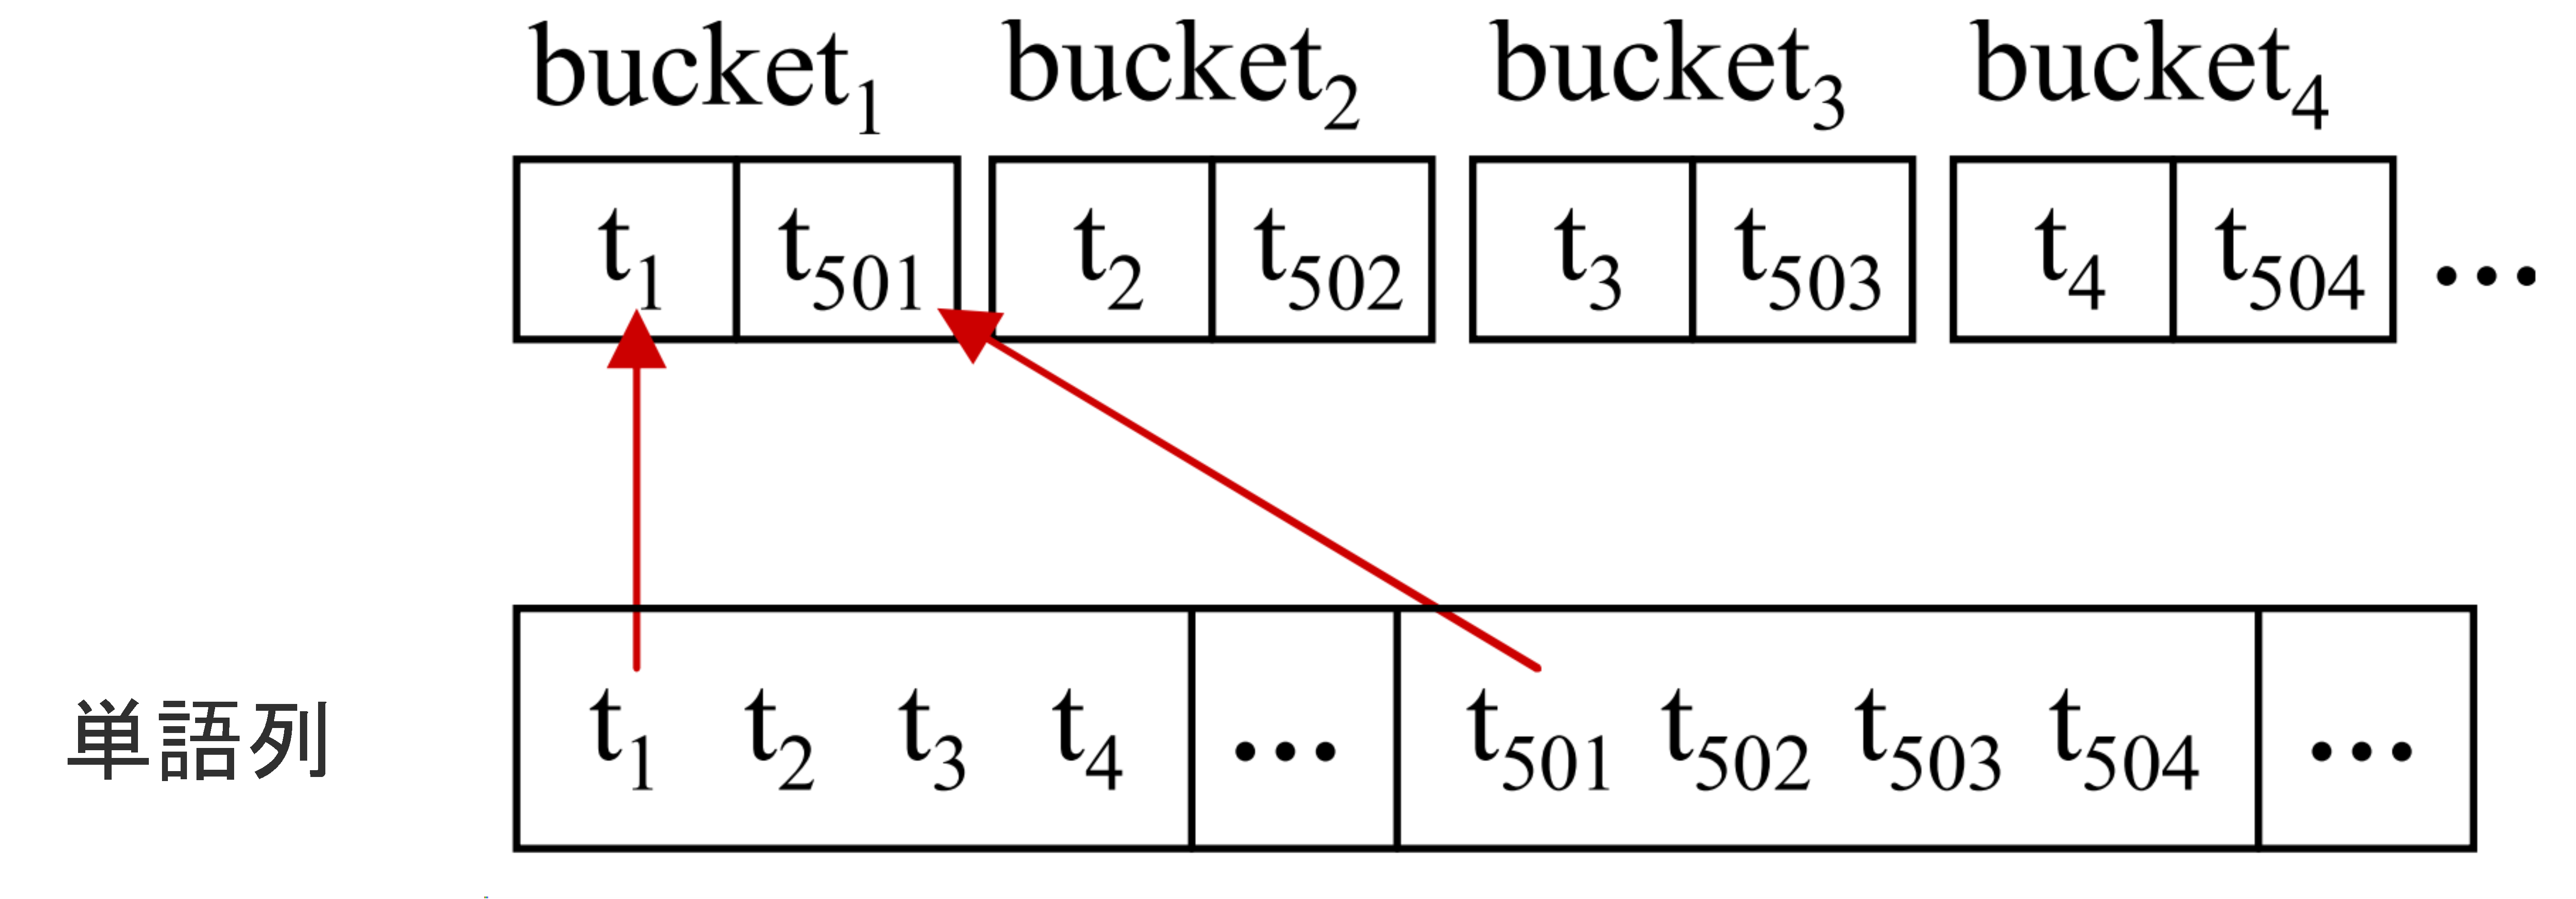
\includegraphics[width=0.8\textwidth,natwidth=5677,natheight=1982]{rk11.png}
	\caption{バケツ作り-$N=1000,BktSz=2$}\label{fig:pp1}
\end{figure}

\begin{algorithm}
\caption{単語列から単語バケツを作る}
\begin{algorithmic}[1]
\Function{GenerateBuckets}{sq,BktSz,Segsz}
	\State $N=$単語列$sq$の長さ
	\State $\#Seg=N/SegSz$
	\State $sq$を同じ長さのセグメントに分割する$S_1,S_2, \dots , S_{\#Seg}$
	\State セグメント中の単語を特殊レベルが大きい方から小さい方への順で再配列する
	\For {$i = 1 to N/(BktSz * SegSz)$}
	\State ActiveSeg = $\phi$
		\For {$j = 1 to BktSz$}
		\State $ActiveSeg = ActiveSeg \cup S_{(j-1)N/(BktSz * SegSz)}$
		\EndFor
		\For {$j = 1 to SegSz$}
		\State 新たなバケツ$B=\phi$を作る
		\State ActiveSeg中の全てのセグメントの$j$番目の単語を$B$に入れる
		\State $B$を出力する
		\EndFor
	\EndFor
\EndFunction
\end{algorithmic}
\end{algorithm}

次ではアルゴリズム1で出力した単語列を単語バケツにする.
アルゴリズム2がその過程を表している.
バケツの大きさを$1 \leq$BktSz$\leq N$に設定すると仮定する.
バケツの数\#Bkts$=N/$BktSz.
同じバケツ中の単語をできるだけ違う意味にするために単語列の$1,\#$BktSz$+1,2*\#$BktSz$+1, \dots,($BktSz$-1)\#$BktSz$+1$番目の単語をバケツ1に,$2,\#$BktSz$+2,2*\#$BktSz$+2, \dots,($BktSz$-1)\#$BktSz$+2$をバケツ2に入れる.
図\ref{fig:pp1}がその過程を表している.
またその操作により,2つのバケツの同じ位置の単語間の距離が一定であり,意味的な距離の差も小さいと考えられる.
したがって,真の質問の単語が意味的に近いときあるいは一つトピックに集中したとき,バケツの中のダミー単語も同じように一つトピックに集中すると考えられる.
しかし,バケツ中の単語の特殊さあるいは特殊レベルがランダムであり,大きく違う可能性がある.

単語の特殊さを調整するために,隣接のバケツ間の単語交換を行う.
図\ref{fig:pp2}がその過程を表している.
実践的には単語列を同じ長さSegSz$\leq N$BktSzのセグメントに分割し,単語を特殊レベルが大きい方から小さい方への順で再配列する.
SegSzがBktSzの整数倍である必要がある.

バケツ作りには2つのパラメータを設定する必要ある.
SegSzが2つのリスクのトレードオフとなる.
SegSzが大きければ大きいほどバケツ中の単語の特殊レベルが近くなる.
一方、単語間の意味的な距離も近く可能性がある.
もう一つパラメータBktSzがプライバシーと計算時間のトレードオフとなる.
BktSzが大きくなると,真の質問を特定する可能性が下がるが,検索エンジンが処理する質問単語が増加する.
SegSzとBktSzを影響は章で述べる.

\begin{figure}
    \centering
    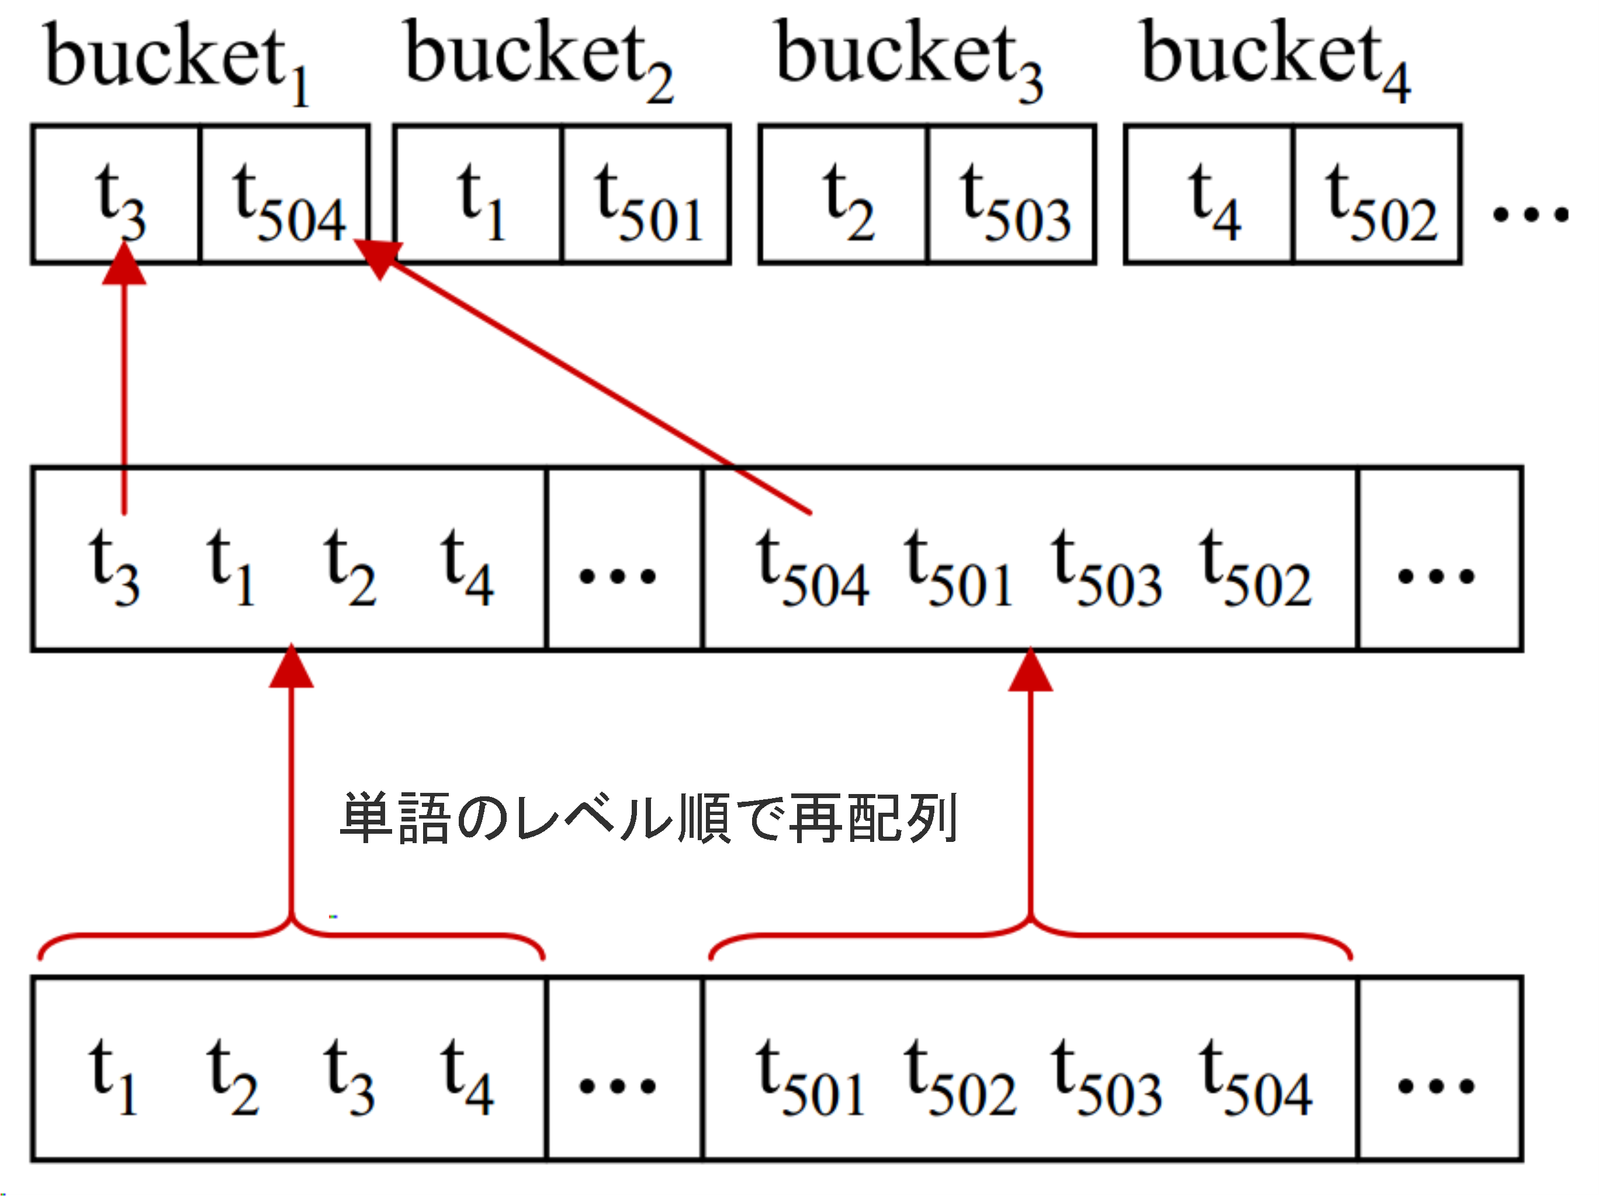
\includegraphics[width=0.5\textwidth,height=0.3\textwidth,natwidth=1600,natheight=1196]{rk13.png}
	\caption{バケツ作り-$N=1000,BktSz=2,SegSz=4$}\label{fig:pp2}
\end{figure}

\subsection{プライベート検索スキーム}
本節では真の質問単語だけの関連性スコアを計算できる検索スキームを述べる.
検索スキームは質問加工,質問検索と結果処理三部分からなる.

\begin{algorithm}
\caption{質問加工}
\begin{algorithmic}[1]
\Function{GenerateBuckets}{sq,BktSz,Segsz}
	\Require 真の質問単語$t_i$の集合
	\Ensure 加工した質問$q$
	\ForAll {真の質問単語$t_i$}
	\State Bkt$=t_i$が属する単語バケツ
		\ForAll {$t_j \in $Bkt}
		\If {$t_i == t_j$} $\mu_j=1$
		\Else $\,\mu_j=0$
		\EndIf
		\State $E(u_j) = g^{\mu_j}\mu^r$
		\State $<t_j,E(\mu_j)>$を$q$に入れる
		\EndFor
	\EndFor
\EndFunction
\end{algorithmic}
\end{algorithm}

アルゴリズム3が質問加工の流れを表す.
真の質問単語が属するバケツの中の他の単語を全てデミー単語として質問に加える.
デミーを加えた質問の単語$t_j$に$E(\mu_j)$を付けつ.
$t_j$が真の質問単語なら$\mu_j=1$,ダミー単語なら$\mu_j=0$.
$E(\cdot)$は\ref{enc}節で紹介した暗号化関数である.
加工した質問$q$をサーバーに送る.

\begin{algorithm}
\caption{質問検索}
\begin{algorithmic}[1]
\Function{GenerateBuckets}{sq,BktSz,Segsz}
	\Require 加工した質問$q$
	\Ensure 文章とその文章暗号文した関連性スコアの集合$R$
	\State $R=\phi$
	\ForAll {$<t_i,E(\mu_i)> \in q$}
		\ForAll {$<d_j,p_{ij}> \in L_i$}
		\If {$\exists <d_j,E(score_j)> \in R$} 
		\State $E(score_j)=E(score_j)*E(\mu_j)^{p_{ij}}$
		\Else 
		\State $<t_j,E(\mu_j)^{p_{ij}}>$を$R$に入れる
		\EndIf
		\EndFor
	\EndFor
\EndFunction
\end{algorithmic}
\end{algorithm}

アルゴリズム4がサーバー側の検索過程を表す.
サーバーが単語と文章の関連値を保存している転置フィルを用いて文章の関連性スコアを計算する.
加算可能な準同型暗号の特徴より,$E(\mu_j)^{p_{ij}}=E(\mu_j*p_{ij})$.
$t_j$がダミー単語であれば,$E(score_j)*E(\mu_j)^{p_{ij}}=E(score_j)*E(0*p_{ij})=E(score_j)$.
復号した関連性スコアには影響を与えない.
したがって,$score_j$が真の質問と文章の関連値$p_{ij}$の和となる.

\begin{algorithm}
\caption{結果処理}
\begin{algorithmic}[1]
\Function{GenerateBuckets}{sq,BktSz,Segsz}
	\Require 文章とその文章暗号文した関連性スコアの集合$R$
	\Ensure 順番順序付けらた文章列
	\State $R=\phi$
	\ForAll {$ <d_j,E(score_j)> \in R$}
		\State $E(score_j)$を$score_j$に復号する
	\EndFor
	\State $R$中の文章を関連性スコアが大きい方から小さい方への順で並べる
	\State $R$中上位の文章を返す
\EndFunction
\end{algorithmic}
\end{algorithm}

最後に質問者がサーバーがらもらった結果集合の関連性スコアを復号し,その値を用いて文章を再配列するとプライバシー保護手法を使っていない検索エンジンと同様な検索結果がもらえる.
アルゴリズム5がこの流れを表している.

\section{メイントピック攻撃}
紹介文献では任意2つのバケツの単語間の意味的な距離の差を小くし真の質問単語間の関連性から真の質問を見破ることを防ぐ.
真の質問が一つトピックに集中したときダミー単語も同じ特殊を表せるかどうかを特許データベース\cite{}を用いて検証した.
単語とトピックの関連性を計算するために\ref{LSI}節で紹介した潜在的意味インデキシングを用いた.
特許文章が表\ref{tab:class}で表したように人手により分類されている.
同じ分類に属する文章を一つの文章を見なし,単語$\cdot$分類行列に潜在的意味インデキシングを行い,文章数が多いコーパスに対応し辛い問題を避けた.

\begin{table}[!hbp]
\center
\begin{tabular}{|c|c|}
\hline
&A61C 5/08A \\
\hline
セクション:A & 健康および娯楽 \\
サブセクション : 61 & 医学または獣医学:衛生学 \\
クラス: C & 歯科:口腔または歯科衛生 \\
メイングループ:5 & 歯の充填または被覆 \\
サブグループ:08 & 歯冠:その製造;口中での歯冠固定 \\
\hline
\end{tabular}
\caption{国際特許分類}\label{tab:class}
\end{table}

\begin{algorithm}
\caption{メイントピック攻撃}
\begin{algorithmic}[1]
	\Require 質問:$Q=\{t_i\},$単語のトピックベクトル集合$L=\{\ell_i\}$
	\State $R=\phi, \, \ell=0$
	\State $\ell=\sum_{t_i \in Q}\ell_{t_i}$
	\State $maintopic=argmax_j \ell[j]$
	\ForAll {$bk_k \in Q $}
	\State $R=R \cup max_{t_i}q_{t_i}[maintopic]$
	\EndFor \\ 
	\Return $R$
\end{algorithmic}
\end{algorithm}

\section{まとめ}


\bibliographystyle{tieice}
\bibliography{zotero}

\end{document}

曖昧化検索(Obfuscation Search)